\documentclass{article}

\usepackage{authblk}
\usepackage{url}
\usepackage[square,numbers]{natbib}
\usepackage{amssymb,amsmath}
\usepackage[margin=1in]{geometry}
\usepackage{graphicx}
\usepackage{setspace}
\doublespacing

%\SectionNumbersOn
%\AbstractOn

\title{A Natural Representation of Functions that Facilitates `Exact Learning'}
%\author{Benedict W. J.~Irwin}


\date{\today}
\begin{document}
%\bibliographystyle{harvard}

%\email{ben.irwin@optibrium.com}
%\affiliation{Optibrium, F5-6 Blenheim House, Cambridge Innovation Park, Denny End Road, Cambridge, CB25 9PB, United Kingdom}
%\alsoaffiliation{Theory of Condensed Matter, Cavendish Laboratories, University of Cambridge, Cambridge, United Kingdom}

\author[1,2]{Benedict W. J.~Irwin}
\affil[1]{Theory of Condensed Matter, Cavendish Laboratories, University of Cambridge, Cambridge, United Kingdom}
\affil[2]{Optibrium Ltd., F5-6 Blenheim House, Cambridge Innovation Park, Denny End Road, Cambridge, CB25 9PB, United Kingdom}
\affil[]{\textit {ben.irwin@optibrium.com}}


\maketitle

\begin{abstract}
We present a collection of mathematical tools and emphasise a fundamental representation of analytic functions. Connecting these concepts leads to a framework for `exact learning', where an unknown numeric distribution could in principle be assigned an exact mathematical description. This is a new perspective on machine learning with potential applications in all domains of the mathematical sciences and the generalised representations presented here have not yet been widely considered in the context of machine learning and data analysis. The moments of a multivariate function or distribution are extracted using a Mellin transform and the generalised form of the coefficients is trained assuming a highly generalised Mellin-Barnes integral representation. The fit functions use many fewer parameters contemporary machine learning methods and any implementation that connects these concepts successfully will likely carry across to non-exact problems and provide approximate solutions. We compare the equations for the exact learning method with those for a neural network which leads to a new perspective on understanding what a neural network may be learning and how to interpret the parameters of those networks.
\end{abstract}

%\tableofcontents

\section{Bigger Picture}
How do we find the mathematical rules behind our data? Many scientific fields have plots, curves and distributions that are not yet assigned an equation. We develop a framework to learn \underline{exact} mathematical solutions from numerical output. This could help researchers solve problems without having to solve equations.
In the long-term, developing such methods could lead to fundamental discoveries about our natural world. Can we learn complicated rules of physics and chemistry by spotting known functions in the data, and from this derive new theories?
We find an analogy between this method and the equations for neural networks that are already used today that gives a new perspective on the meaning of network parameters in existing models and could lead to advances in understandable AI. 



\section{Introduction}
Machine learning (ML) is - simplistically speaking - a form of function fitting and ML methods often try to recreate a set of training observations by fitting a function to - or `learning from' - example data points. For a given problem, the most appropriate ML method to use will depend on the application. In general, great success has been seen using this kind of methodology on a range of problems across all domains of science and industry. Most current ML methods recreate the input data by an approximation or interpolation of a restricted sample of training points. Any learning that happens by these methods is then also in some sense restricted or limited to the domain of the training set or conditions in which the data were collected. The form chosen to fit the data - the model - is usually selected for convenience, convergence properties, speed, or simplicity and interpretability and the coefficients/weights/parameters learned are likely to be somewhat arbitrary, not necessarily represent anything fundamental, and become much harder to interpret as the method gets increasingly complex \cite{Carvalho2019}. In order to reach these high precision approximations, many parameters are used, sometimes millions or billions of parameters, especially in the case of neural networks and deep learning methods \cite{Lecun2015}.\\


The trained model from the above methods is unlikely to be `physically meaningful', by which we mean - unlikely to lead to transparent and understandable insight that can be condensed down into a human readable form. The \emph{outputs} of the model can still be very useful, for example to interpolate between known physical results \cite{Belisle2015}, but the model itself is not necessarily fundamental. This makes it hard for current ML methods to assist in the collection of fundamental things, or `natural facts', specifically mathematical facts. True learning - in a mathematical sense - is timeless. If an exact solution to a problem exists - for example a solution to a particular differential equation - this solution is a permanent solution which can be defined,  collected, and documented in a human readable form\footnote{Subject to the language required to document the function existing.}. If the same equation is written years in the future the same solution will apply. Learning such a fact correctly would then be an example of `\emph{exact learning}'. This notion is more relevant to problems from mathematics and physics where there is an unchanging `ground truth' defined by nature, for example laws of physics. \\


We will consider how in a broad sense `machine-learning-like-techniques' (i.e. advanced function fitting), can help with these `exact learning' type problems. Specifically for this work, the problem description is: 
\begin{enumerate}
\item[A)] \textbf{`Given a high precision numeric output of an unknown multivariate function or distribution write the `human readable equation' for that function as output, where it is possible to do so."}
\end{enumerate}
The concession we are willing to take on this quite general goal is:
\begin{enumerate}
\item[B)] \textbf{`Given a high precision numeric output of an unknown multivariate distribution write the \emph{unique fingerprint} of the distribution.'}
\end{enumerate}

The key change in goal B) is the introduction of a `\emph{fingerprint}' of an arbitrary function as a well behaved and meaningful intermediate that can identify a distribution \footnote{We have focused on distributions for the time being for simplicity, but extensions to this method will cover functions which are not bound at infinity}. The word fingerprint is local to this text and should not be considered a general term. The goals A) and B) can be seen as reverse engineering processes for \emph{functions}. It might be helpful to first consider the analogy of reverse engineering for a simpler object such as a \emph{number}, something that is performed by tools such as Simon Plouffe's `inverse symbolic calculator' \cite{Plouffe1986} and other `inverse equation solvers' \cite{Munafo}. In these tools a user can enter a high precision number - e.g. 14.687633495788080676 - and the algorithm would return a plausible closed form solution - e.g. $\pi^2 + e\sqrt{\pi}$. Once the user has the solution, the hope is that a human expert could use that extra information to come up with further insights which would assist in the scientific understanding of both the solution and problem.\\ 

Figure \ref{fig:Outline} depicts an overview of the `exact learning' procedure for a \emph{function}. Throughout this work we cover the necessary tools to understand the steps in the blue boxes on the right-hand side of this figure. Goal A) corresponds to the bottom left box, and goal B) is the bottom right box. The numeric data are collected from a natural source such as a very high-quality experiment, but more likely a numerical solution to a computational problem, or equation, or simulation. The solution is numerically transformed to `fingerprint space' (blue) by using an integral transform. The regularity of the representation of many analytic functions in this space assists with the fitting of the `fingerprint' using machine learning techniques to an assumed, highly generalised form. To get back to the mathematical expression of the solved function an inverse transformation is taken from the  fingerprint space to the function space. For examples of problems that might be interesting to solve using this method, please refer to the supplementary information. \\

\begin{figure}[h]
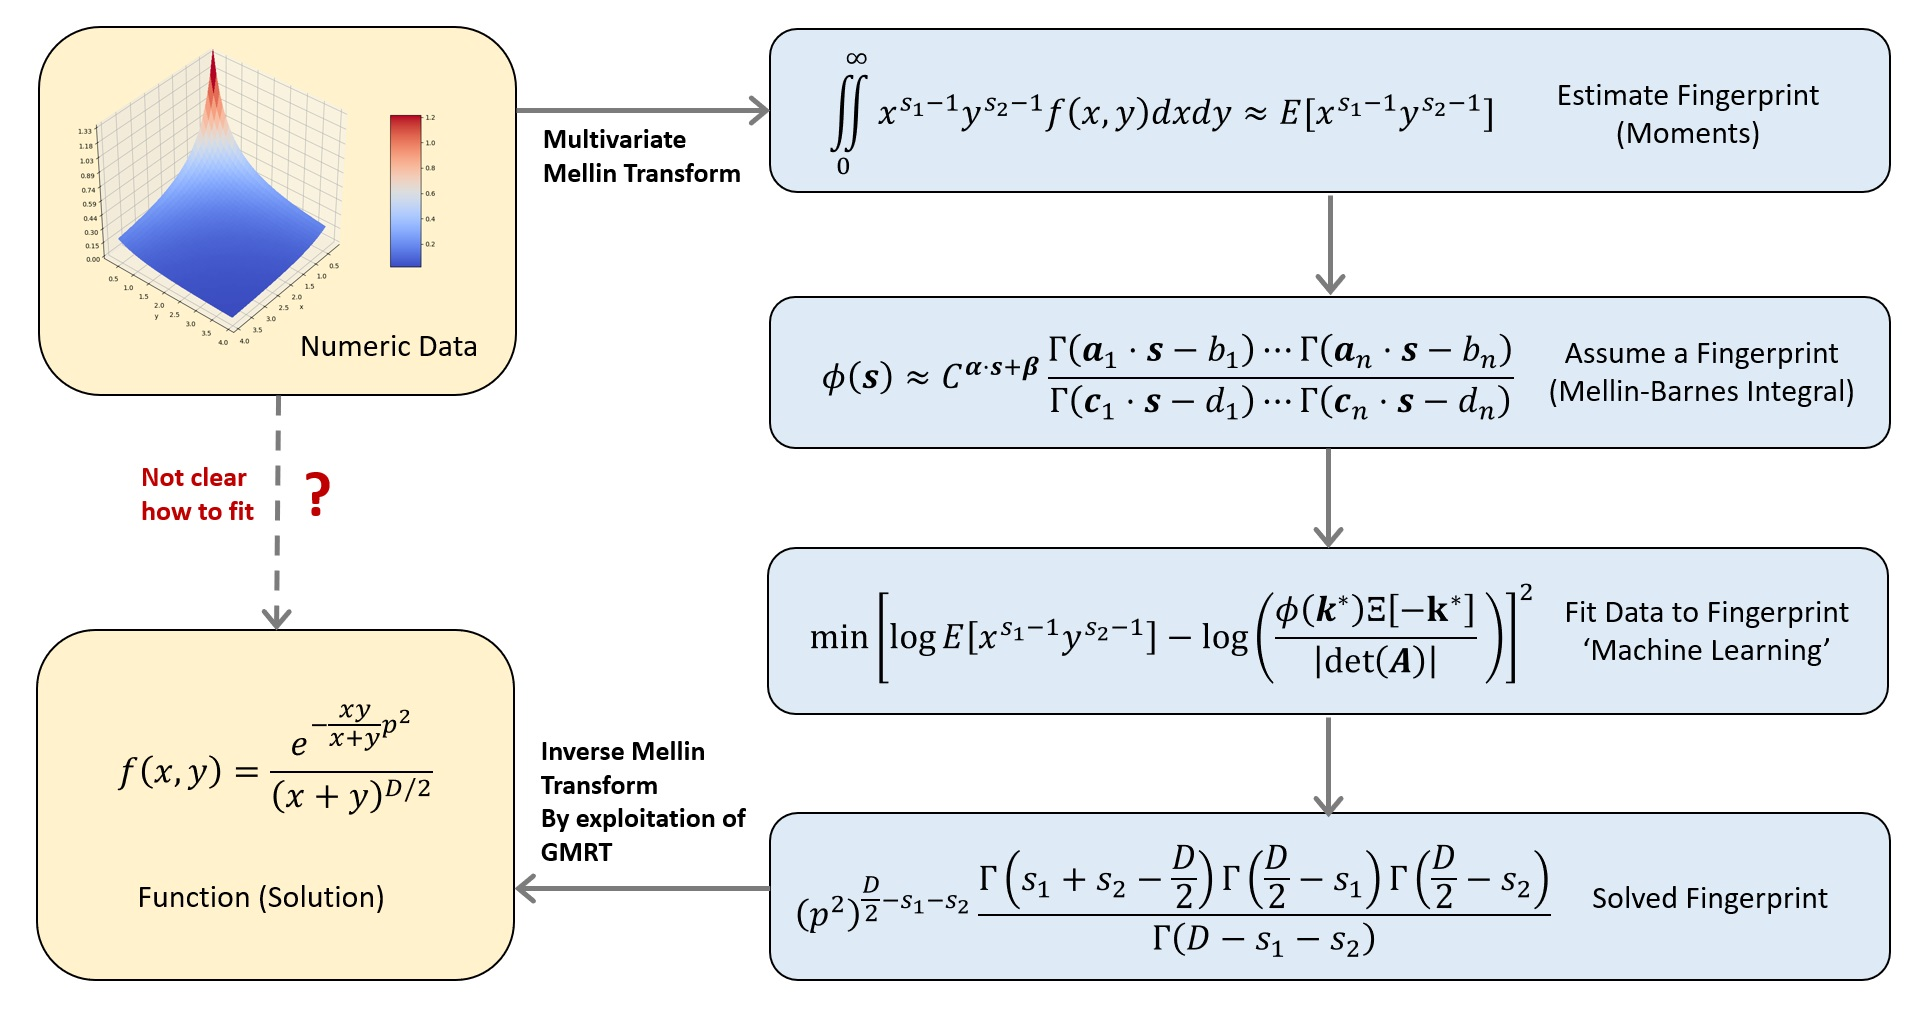
\includegraphics[scale = 0.323]{Figure1.jpg}
\caption{An example of the exact learning process, in this case with an example of the kernel of the massless Feynman bubble calculation given by Gonzalez et al. \cite{Gonzalez2015}. (Top left), A high precision numerical function is found as the solution to a problem that likely has an analytic solution, but the closed form is hard to derive mathematically. A numeric Mellin transform is made from the `function domain' (yellow) into the `fingerprint domain' (blue) for a number of chosen exponent vectors $\mathbf{s}=(s_1,\cdots,s_2)$. A highly generalised closed form for the fingerprint is chosen and then machine learning (function fitting) is used to track down the parameters of the function fingerprint ($\mathbf{a,b,c,d}$). With further analysis and interpretation of the solved parameters the fingerprint could be used to derive the closed form for the function that generated the original numeric data using the generalised Ramanujan master theorem (GMRT).}
\label{fig:Outline}
\end{figure}

\subsection{Brief Disclaimer}
This intends to be a foundational paper that sparks an idea and lays the concepts on the table but stops short of connecting them together. This is to avoid invoking (an explanation of) the technical requirements that are needed for an implementation. Many of the tools described here are treated in a highly rigorous mathematical way in the literature. While this is necessary for the correctness of the underlying mathematics, we feel it reduces the accessibility of the concepts, innovation, and creativity. We will introduce the necessary fundamentals with a high level overview and point to more technical references where possible. \\

There are a number of limitations and potential `engineering problems' that may need to be overcome when training networks that are constructed using these concepts introduced below. For a further discussion of limitations please see the supplementary information. Further work is undoubtedly required to overcome these issues and some of these are discussed with the conclusions. The key message of this work is: `Let us turn our attention to a special hierarchy of functions and associated methods while keeping machine learning in mind. What algorithms can be developed from this?'.


\section{Background and Method}
We will go through the background theory and arrangement of concepts required to exactly learn functional forms from high-quality numeric data. As with other types of machine learning, fitting and optimisation problems, it is convenient to define a loss function that should be minimised to solve the problem \cite{Rosasco2004}. If this loss function takes a standard form, there are many available minimisation methods, for example using the gradient of the loss function with respect to network parameters \cite{Ruder2016}. The training process for a method built using the loss function would then resemble backpropagation for a (deep) neural network \cite{Wang2017,Lecun2015} and completed algorithm is more likely to be implementable with existing software packages such as TensorFlow \cite{Abadi2016} and PyTorch \cite{Paszke2019}. Other learning strategies may prove more efficient or robust \cite{Greenfeld2019}.\\
 
For the time being, this conceptual loss function will be the squared difference of the `experimental fingerprint' of the numerical solution, after the transformation into fingerprint space, and the `theoretical fingerprint' i.e the model we are trying to fit to the data. We then answer the questions: `What is the fingerprint of a function?' and `How do we measure this fingerprint both experimentally and theoretically?'. The fingerprint we choose in this work is the so-called \textbf{Mellin transform} of a function or distribution \cite{Fikioris2006}. To understand the rationale behind choice this we first explain a pattern in the generalised representation of analytic functions which we believe to be fundamental.


\subsection{Nature's Language for Analytic Functions}
Many different types of mathematical function are used across the mathematical sciences. Because the language of mathematics is an \emph{ad hoc} set of notation which has evolved with time it can be hard to keep a sense of order on named functions. Many people will be familiar with the functions $\exp(x)$ and $\log(x)$, which seem fundamental to nature, or trigonometric functions such as $\sin(x)$. In engineering and physics yet more complicated special functions were developed for convenience, e.g. Bessel functions which can relate to cylindrical harmonics, along with various special (orthogonal) polynomials and these functions and identities appear in large catalogues \cite{Kolbig1995}. \\

The subset of \emph{analytic functions} have power series expansions which allow easier comparison between functions. Many of these series expansions can represented in terms of so-called \textbf{hypergeometric series}. A a core-component of this description is the gamma function
\begin{equation}
\Gamma(s) = \int_0^\infty x^{s-1} e^{-x}dx,
\end{equation}
which is the continuous analogue to the factorial function $n!$ \cite{Fikioris2006,Kolbig1995}. The gamma function will be pivotal for our definition of a function's fingerprint. We also not that $s$ should generally be considered a complex number.\\

Functions that can be described as a hypergeometric series can be represented as a limiting case of the so-called \textbf{hypergeometric function} which can be written in terms of ratios of gamma functions. We can write the hypergeometric function (with a negative argument) as
\begin{equation}
_2F_1(a,b;c;-x) = \sum_{s=0}^\infty \frac{(-1)^s}{s!} \frac{\Gamma(c)\Gamma(a+s)\Gamma(b+s)}{\Gamma(a)\Gamma(b)\Gamma(c+s)} x^s,
\label{eqn:hypergeom}
\end{equation}
where the notable component is the collection of gamma functions in the series. In this work we define the \emph{fingerprint} of the hypergeometric function as the so-called \textbf{Mellin transform} \cite{Fikioris2006} of the function, 
\begin{equation}
\mathcal{M}\left[_2F_1(a,b;c;-x)\right](s) = \underbrace{\frac{\Gamma(c)\Gamma(a-s)\Gamma(b-s)\Gamma(s)}{\Gamma(a)\Gamma(b)\Gamma(c-s)}}_{fingerprint},
\end{equation}
which is related to the series coefficients in equation \ref{eqn:hypergeom}. For a large set of analytic functions used in science and mathematics, \textbf{the fingerprint is described as a product of Gamma functions and their reciprocals}. This scrathes the surface of the fundamental pattern we will exploit to allow machine learning methods to adapt to unknown functions. For more examples of the Mellin transform and for a list of example functions from science and mathematics that can be described by hypergeometric series and increasingly generalised series see the supplementary information. \\

Many analytic functions \emph{cannot} be described by the simple hypergeometric series in equation \ref{eqn:hypergeom} \cite{Rathie1997}. There are further extensions to the series definition which begin to describe these additional functions. This process of generalisation has iterated numerous times over the course of history \cite{Wright1935,Fox1961,Inayat-Hussain1987,Rathie1997}, each time capturing successively more of the functions which are not described by the previous iterations. It is this neat and hierarchical way of organising this huge space of functions which we will use as a language for `exact learning'. The latest and more complex iterations have provided functions which can describe complex phenomena from physics such as the free energy of a Gaussian model of phase transition \cite{Rathie1997}. We will briefly describe the language used to define these highly generalised functions.\\

\subsubsection{A Language to Define Analytic Functions}
The Mellin transform converts a function into its fingerprint and the \textbf{inverse Mellin transform} transforms the fingerprint into the function. The inverse Mellin transform is defined by a contour integral, that uses the residue theorem to recreate the series expansion of the function \cite{Fikioris2006,Mainardi2003}. The more generalised functions considered in this work are \emph{defined} in terms of this contour integral \cite{Rathie1997,Rathie2013,Rathie2018}, which is often called a \textbf{Mellin-Barnes integral} \cite{Mainardi2003}. For the hypergeometric function (Equation \ref{eqn:hypergeom}) a corresponding definition through a Mellin-Barnes integral is
\begin{equation}
_2F_1(a,b;c;-x) =\frac{1}{2\pi i} \int_{-i\infty}^{i\infty} \frac{\Gamma(c)\Gamma(a+s)\Gamma(b+s)\Gamma(-s)}{\Gamma(a)\Gamma(b)\Gamma(c+s)}x^s\,ds.
\label{eqn:contour1}
\end{equation}
there are technical reasons for this choice of languge over a simpler series representation. For example a different choice of contour can lead to different representations of a series \cite{Rathie1997}, other methods to compute Mellin transforms find multiple ways of getting to the same answer \cite{Gonzalez2015}. We will not dive into the technical details, but present equation \ref{eqn:contour1} to observe that the contents of this Mellin-Barnes integral is simply the fingerprint, with a change of sign $s \to -s$. 

\subsubsection{A Fundamental Duality}
The duality between a function and its Mellin transform has proved useful in numerous advanced mathematical applications including quantum field theory \cite{Gonzalez2015}, cosmology \cite{Sleight2020}, and string theory \cite{Passare1996}. Schwinger and Feynman parametrisation for the calculation of loop integrals from Feynman diagrams make heavy use of Mellin transforms \cite{Sameshima2019} and the resulting `Mellin space' has been viewed as a `natural language' for attempts to align quantum gravity and quantum field theory in Ads/CFT methods \cite{Fitzpatrick2011}. It is possible to convert the regular Fourier duality\footnote{Position and momentum, and time and frequency form conjugate pairs of variables.} of quantum mechanics into a `Mellin duality', which leads to wavefunctions associated with the zeta functions commonly seen in number theory \cite{Twamley2006}. Aspects of particle physics have also previously been noted in the analytically continued coefficient space of zeta type functions \cite{Woon1997}. Therefore, it is not out of the question that the Mellin transform representation of the `fingerprint' also be a natural choice for exact learning. This representation is the frame in which functions are defined by their zeroes and poles, in the same way that many properties of prime numbers are defined by the zeroes of the Riemann zeta function. \\

There is a simple relationship between the Fourier transform $\mathcal{F}$, the (two-sided) Laplace transform $\mathcal{L}$ and the Mellin transform $\mathcal{M}$ for a function $f$. Namely, the Mellin transform of a function $\mathcal{M}[f(x)](s)$ is the same as the Laplace transform of the same function with negative exponential argument, $\mathcal{L}[f(e^{-x})](s)$, which is related to the Fourier transform as $\mathcal{F}[f(e^{-x})](-is)$, and likewise the Fourier transform of a function $\mathcal{F}[f(x)](-s)$, relates to $\mathcal{L}[f(x)](-is)$ and to $\mathcal{M}[f(-\ln x)](-is)$.\\

Dualities in these other two transform spaces have been known for a long time to statistics including the relationship between the characteristic function and the distribution in terms of a Fourier transform \cite{Waller1995}, and the moment generating function and a distribution in terms of the Laplace transform \cite{Spataru2007}. However, in terms of \emph{fingerprint equivalents}, Laplace and Fourier transforms do not display the regularity of the Mellin transforms in terms of patterns of gamma functions alluded to in the above sections. This can be seen by reviewing extensive tables of each type of transform \cite{Bateman1953}. Many of the identities for Fourier transforms relate to trigonometric functions and Bessel functions and many of the Laplace transform identities relate to algebraic expresions and exponential terms. Both Fourier and Laplace transforms make extensive use of special functions such as error functions, exponential integrals and more complicated, niche special functions. On the other hand, the Mellin transform identities mostly revolve around gamma functions and polygamma functions, hypergeometric functions and terms such as beta functions and other shorthands which can actually be expressed again as gamma functions e.g. $\pi \csc(\pi s)=\Gamma(s)\Gamma(1-s)$. Loosly speaking, these `elements' that form the Mellin transforms all have something to do with gamma functions. \\


The Mellin transform connects a distribution to its moments, and learning using moments has been considered before, including the generalised method of moments \cite{Zsohar2012}. These methods do not consider an underlying structure to the moment space, but only that estimators of statistical quantities phrased in terms of moments can be advantageous. In general integral transforms link strongly to inner products in vector spaces and further work would be required to establish a deep connection between `exact learning' as presented here to well studied mathematical formalisms such as a reproducing kernel Hilbert spaces \cite{Wahba2003}, specifically those with a monomial kernel $x^s$ as seen in the Mellin transform. Further much deeper mathematical connections are apparent, including the generalisation of the Mellin transform in terms of a Gelfand transform, or the analogies between hypergeometric functions and `basic hypergeometric', `q-hypergeometric' and elliptic variants \cite{Thakur1991}.\\

To summarise, the Mellin transform can mediate a duality between a distribution and its moments, or an analytic function and its coefficients in the same way that a Fourier transform can mediate a duality between time and frequency, or position and momentum. In terms of function fitting, an analytic function represented as a power series has infinite coefficients to fit, however, by applying the Mellin transform the coefficients are not trained individually but the whole set of coefficients are trained simultaneously. 


\subsubsection{Generalisation of Generalised Functions}
For the generalised functions beyond the hypergeometric function, the product of gamma functions that forms the fingerprint begins to have numerous terms and it is helpful to define a concise notation for a `product gamma' operation, $\Xi[\cdot]$, which flattens a vector or matrix and takes a product of the gamma function over the elements. The use of this custom operation will make the pattern between the functions much easier to see. Table \ref{tab:Xi} shows how the operation works for vector and matrix arguments and includes an optional vector $\mathbf{v}$ (or matrix $\mathbf{V}$) of exponents of equal size to realise `products of powers of gamma functions'. This can be easily extended for any array or tensor of higher dimensions.
\begin{table}[h]
\caption{Table explaining the $\Xi[\cdot]$ operation on different inputs with and without vector or matrix arguments and exponents. The argument and exponent should be of the same size and shape.}
\centering
\begin{tabular}{|c|c|c|}
\hline
Input & Vectors $\mathbf{a,v} \in \mathbb{R}^D$ & Matrices $\mathbf{A,V} \in \mathbb{R}^D\times \mathbb{R}^D$ \\
\hline
No Exponent & $\Xi[\mathbf{a}] = \prod_{k=1}^D \Gamma(a_k)$ & $\Xi[\mathbf{A}] = \prod_{k=1}^D\prod_{l=1}^D \Gamma(A_{kl})$ \\
Exponent & $\Xi^\mathbf{v}[\mathbf{a}] = \prod_{k=1}^D \Gamma^{v_k}(a_k)$ & $\Xi^\mathbf{V}[\mathbf{A}] = \prod_{k=1}^D\prod_{l=1}^D \Gamma^{V_{kl}}(A_{kl})$\\
\hline
\end{tabular}
\label{tab:Xi}
\end{table}

The hierarchy of the highly generalised series that go beyond the simple hypergeometric series is presented in table \ref{tab:main} with the function name and notation along with and the associated Mellin transform (i.e. the fingerprint). In order to make the similarities clear, as well as using the compact $\Xi$ notation, we have slightly altered the notation for input parameters on some of the functions. In all cases beyond the hypergeometric function the inputs are \emph{vector} quantities and the scalar indices $p,q,m,n$ denote the lengths of input vectors according to the function definition. The progression in terms of complexity - and therefore flexibility to represent more functions - advances down the table. We start with the hypergeometric function \cite{Kolbig1995,Fikioris2006} and its generalisation \cite{Kolbig1995}, the Fox-Wright series and its normalised counterpart \cite{Wright1935}, the highly flexible Meijer-G function \cite{Bateman1953} and its analogous extension the Fox-H function \cite{Fox1961}. We include two more recent, extremely general extensions, the Inayat-Hussain-$\bar{H}$ \cite{Inayat-Hussain1987} and the Rathie-I function \cite{Rathie1997}. We note that Rathie has also extended to even more generalised functions \cite{Rathie2013} which are briefly discussed in section `Analogy to Deep Networks'. Table \ref{tab:main} is not necessarily exhaustive, for example functions such as the MacRobert-E function \cite{MacRobert1962} are not represented. These functions bridge the gap between hypergeometric and Meijer-G type functions which are separated by a horizontal divide in the table, the distinguishing feature is a free $\Gamma(s)$ term in the Mellin transform and a requirement to negate the argument of the function for hypergeometric type series for comparison. For all functions, a simple scale factor $\eta$ has been included to demonstrate that this appears as a simple power in the fingerprint due to the properties of the Mellin transform. The Meijer-G function suffers from an unfortunate notation where the vectors of parameters are split. It is convenient to rewrite the two vectors of parameters, as four individual vectors of parameters for a consistent hierarchy.\\

The hierarchy in table \ref{tab:main} progresses in terms of complexity by starting with scalar shift parameters $a,b,c$ in the arguments of the gamma functions. Then the number of gamma functions is increased, and vector shift parameters $\mathbf{a,b,c,d}$ are used. We switch to the $\Xi$ notation from table 1 at this point to retain compact expressions. Next the inclusion of vector scale parameters, $\mathbf{e,f,g,h}$, extend from hypergeometric functions to Meijer-G functions, which gives a large boost to the types of function that can be represented. The most general functions come from adding vector power parameters $\mathbf{i,j,k,l}$, which begin to describe non-trivial physical and number theoretic functions \cite{Rathie1997}.

\begin{table}
\caption{A table of generalised special functions and their Mellin transforms. Small bold letters are vectors of parameters where $\mathbf{a,b,c,d}$ are shift factors, $\mathbf{e,f,g,h}$ are scale factors and $\mathbf{i,j,k,l}$ are exponents for the gamma functions, $\mathbf{1}$ represents a vector containing only 1's. Complexity increases down the table which is split into an upper part for hypergeometric functions and a lower part for Meijer-G like functions.}
\centering
\begin{tabular}{|p{2.3cm}|c|p{3.5cm}|c|}
\hline
Function \newline Name & $f(x)$ & Fingerprint \newline $\varphi(s)=\mathcal{M}[f(x)](s)$ & Ref. \\
\hline
Hypergeometric & $_2 F_1 \!\left( \left. \begin{matrix} a,b \\ c \end{matrix} \; \right| \, -\eta x \right)$ & $\eta^{-s}\frac{\Gamma(c)\Gamma(a-s)\Gamma(b-s)}{\Gamma(a)\Gamma(b)\Gamma(c-s)}\Gamma(s)$ & \cite{Kolbig1995,Bateman1953}\\
Generalised \newline Hypergeometric &  $_p F_q \!\left( \left. \begin{matrix} \mathbf{a} \\ \mathbf{b} \end{matrix} \; \right| \, -\eta x \right)$ & $\eta^{-s}\frac{\Xi[\mathbf{b}]\Xi[\mathbf{a}-s\mathbf{1}]}{\Xi[\mathbf{a}]\Xi[\mathbf{b}-s\mathbf{1}]}\Gamma(s)$ &  \cite{Kolbig1995,Bateman1953}\\
Fox-Wright-$\Psi$ & $_p\Psi_q \!\left[\left.\begin{matrix}
\mathbf{a},\mathbf{e} \\
\mathbf{b},\mathbf{f} \end{matrix} \;\right| -\eta x  \right]$ & $\eta^{-s}\frac{\Xi[\mathbf{a}-s\mathbf{e}]}{\Xi[\mathbf{b}-s\mathbf{f}]}\Gamma(s)$ & \cite{Wright1935}\\
Fox-Wright-$\Psi^*$ & $_p\Psi_q \!\left[\left.\begin{matrix}
\mathbf{a},\mathbf{e} \\
\mathbf{b},\mathbf{f} \end{matrix} \;\right| -\eta x  \right]$ & $\eta^{-s}\frac{\Xi[\mathbf{b}]\Xi[\mathbf{a}-s\mathbf{e}]}{\Xi[\mathbf{a}]\Xi[\mathbf{b}-s\mathbf{f}]}\Gamma(s)$ & \cite{Wright1935}\\
\hline
Meijer-G & $G_{p,q}^{\,m,n} \!\left( \left. \begin{matrix} \mathbf{a,b} \\ \mathbf{c,d} \end{matrix} \; \right| \, \eta x \right)$ & $\eta^{-s}\frac{ \Xi[\mathbf{1}-\mathbf{a}-s\mathbf{1}]\Xi[\mathbf{c}+s\mathbf{1}]} {\Xi[\mathbf{1}-\mathbf{d}-s\mathbf{1}]\Xi[\mathbf{b}+s\mathbf{1}]}$& \cite{Bateman1953,Mainardi2003}\\
Fox-H & $H_{p,q}^{\,m,n} \!\left[\left. \begin{matrix}
\mathbf{a},\mathbf{b},\mathbf{e,f} \\
\mathbf{c},\mathbf{d},\mathbf{g,h} \end{matrix} \right| \eta x \right]$ & $\eta^{-s}\frac{\Xi[\mathbf{1-a}-s\mathbf{e}]\Xi[\mathbf{c}+s\mathbf{g}]}{\Xi[\mathbf{1-d}-s\mathbf{h}] \Xi[\mathbf{b} + s \mathbf{f}]}$ & \cite{Fox1961,Rathie2018}\\
Inayat-Hussain-$\bar{H}$  & $\bar{H}_{p,q}^{\,m,n} \!\left[\left. \begin{matrix}
\mathbf{a},\mathbf{b},\mathbf{e,f,i} \\
\mathbf{c},\mathbf{d},\mathbf{g,h,l} \end{matrix} \right| \eta x \right]$ & $\eta^{-s}\frac{\Xi^{\mathbf{i}}[\mathbf{1-a}-s\mathbf{e}]\Xi[\mathbf{c}+s\mathbf{g}]}{\Xi^{\mathbf{l}}[\mathbf{1-d}-s\mathbf{h}] \Xi[\mathbf{b} + s \mathbf{f}]}$ & \cite{Inayat-Hussain1987}\\
Rathie-I & $I_{p,q}^{\,m,n} \!\left[\left. \begin{matrix}
\mathbf{a},\mathbf{b},\mathbf{e,f,i,j} \\
\mathbf{c},\mathbf{d},\mathbf{g,h,k,l} \end{matrix} \right| \eta x \right]$ & $\eta^{-s}\frac{\Xi^{\mathbf{i}}[\mathbf{1-a}-s\mathbf{e}]\Xi^{\mathbf{k}}[\mathbf{c}+s\mathbf{g}]}{\Xi^{\mathbf{l}}[\mathbf{1-d}-s\mathbf{h}] \Xi^{\mathbf{j}}[\mathbf{b} + s \mathbf{f}]}$ & \cite{Rathie1997}\\
\hline
\end{tabular}
\label{tab:main}
\end{table}

All of the functions in table \ref{tab:main} assume an analytic series expansion. For certain sets of parameters, the series expansions for many commonly used functions in physics and mathematics can arise. A small list is given in the supplementary information. Many of these functions have constraints on the combinations of arguments that can be used. For the sake of focus and scope in this text we will not mention any regions of convergence or the necessary analytic continuations in the following sections, but these should be considered carefully when such equations are implemented numerically and solved fingerprints are interpreted. A careful treatment is given by the following references \cite{Geenens2017,Passare1996,Peasgood2009} as well as the reference for each function in table \ref{tab:main}.\\

Work has already been done to harness the flexibility of this relationship to cover a wide space of functional forms. Geenens  derives a particular kernel density estimator \cite{Geenens2017} using the Meijer-G function and its Mellin transform, which can capture as limiting cases a number of common statistical distributions over a one dimensional domain, including beta prime, Burr, chi, chi-squared, Dagum, Erlang, Fisher-Snedecor, Frechet, gamma, generalised Pareto, inverse gamma, Levy, log-logistic, Maxwell, Nakagami, Rayleigh, Singh-Maddala, Stacy and Weibull distributions \cite{Geenens2017}. This is already testament to the potential power behind this representation. Geenens also gives an excellent summary of the mathematical properties of the Mellin transform and its applications to probability functions and some of the more technical details and important considerations surrounding the Meijer-G function itself \cite{Geenens2017}. \\

The take away point is that all of the functions in this natural hierarchy can be defined as a Mellin-Barnes integral in the form
\begin{equation}
f(x) = \frac{1}{2\pi i}\int_L z^s \bar{\phi}(s)\;ds,
\label{eqn:contour}
\end{equation}
for a suitable definition of $\bar{\phi}$ \cite{Rathie1997}. $L$ is a special contour path which is covered in detail in references defining each function. The fundamental pattern is that for all of these generalised functions $\bar{\phi}$ is expressed as a product of gamma functions and their reciprocals. The contour $L$ encircles poles which contribute to the series expansion of $f(x)$. The function $\bar{\phi(s)}$ is related to the Mellin transform - and therefore the fingerprint - of $f(x)$ by inverting the sign of $-s$. Thus, if we assume a highly generalised \textbf{theoretical fingerprint} which is a product of gamma functions and their reciprocals, with shift, scale and power parameters, we can recreate a flexible subset of the analytic function space for a general and unknown function $f(x)$. \\


\subsection{Ramanujan Master Theorem (RMT)}
We have identified the Mellin transform is the method of extracting the fingerprint of a function. The goal of this work was to identify an unknown function from numeric data. Now we can assume a generalised theoretical fingerprint of a form from table \ref{tab:main} to define the desired level of complexity. Then we train the parameters in the theoretical fingerprint to reveal the function's definition. In order to do this we will elaborate on the following additional steps: \begin{enumerate}
\item[1)] Numerically perform the Mellin transform to convert numeric function data to numeric `fingerprint' data.
\item[2)] Fit the function fingerprint (machine learning techniques).
\item[3)] Reconstruct the function from its fingerprint.
\end{enumerate}
Point 1) is relatively easily obtained for distributions by interpreting the definition of the Mellin transform as the `moments' of a probability distribution. We can approximate for a set of well sampled data points $x_i \in \{x\}$ and $x_i \sim P(x)$,
\begin{equation}
\mathcal{M}[P(x)](s) = \int_0^\infty x^{s-1} P(x) \; dx = E[x^{s-1}] \approx \frac{1}{N}\sum_{k=1}^N x_k^{s-1},
\end{equation}
and where this is not applicable for reasons of bias and sampling, there is existing theory of unbiased estimators that can be invoked to extract moments \cite{Zsohar2012}. The key point here is that we must sample the moments at a number of values of exponent $s$. For advanced treatments these may need to be real, fractional or even complex numbers, because the fingerprints are often defined for inputs from the complex plane. For functions which are not distributions, we require an equivalent process of extracting the coefficients numerically. For this numerous numeric Mellin transform algorithms exist.\\


For point 2) there already exists a number of strategies for training models and networks. There are gradient methods such as those used in deep learning \cite{Lecun2015,Kingma2015,Ruder2016}, or stochastic sampling methods over parameters, and potentially advanced constructive techniques \cite{Greenfeld2019}. One would minimise the square difference between the numeric fingerprint extracted using point 1) and the theoretical fingerprint selected from table \ref{tab:main}. Due to the rapidly growing nature of gamma functions it is useful to instead minimise the square \emph{log difference} of the numeric and theoretical fingerprints. The resulting sum of log-gamma functions has an interesting interpretation and mathematical properties and this is discussed in section "Comparison to a Neural Network".\\

For point 3) we come back from the fingerprint domain into the function domain (i.e. the inverse Mellin transform). The bridge we use to skip between domains is called the \textbf{Ramanujan Master Theorem} (RMT) \cite{Amdeberhan2012}, which offers a deeper understanding of the meaning of the fingerprint of a function. For suitable functions that admit a series expansion of the form
\begin{equation}
f(x) = \sum_{k=0}^\infty \chi_k \phi(k)x^k, \;\;\;\;\; \chi_k = \frac{(-1)^k}{k!}
\label{eqn:RMTSum}
\end{equation}
where $\chi_k$ can be considered an `alternating exponential symbol' \footnote{If $\sum_i a_ix^i$ is a generating function and $\sum_i \frac{a_ix^i}{i!}$ is an \emph{exponential} generating function and if $\sum_{i} a_i$ is a sum and $\sum_i (-1)^i a_i$ is an \emph{alternating sum} it makes sense to call $\frac{(-1)^i}{i!}$ the alternating, exponential symbol.} the RMT simply states that the Mellin transform of the function is given by
\begin{equation}
\mathcal{M}[f(x)](s) = \Gamma(s)\phi(-s)
\label{eqn:RMT}
\end{equation}
where $\Gamma(s)$ is the gamma function. This relationship sometimes relies on the \textbf{analytic continuation} of the coefficient function $\phi(s)$ to accept negative (and potentially complex) quantities. Functions whose $\phi(k)$ coefficients are products of gamma functions and their reciprocals are generally well behaved under continuation to the entire complex plane due to $\Gamma(s)$ being an almost entire function. This relationship holds very successfully for functions which admit definition through a Mellin-Barnes integral which is true of all of the functions in table \ref{tab:main}. \\

Contour integrals of the form in Equation \ref{eqn:contour} are notoriously hard to work with in numerical algorithms. The RMT acts as a (two way) bridge that lets us avoid contour integrals of the type in equation \ref{eqn:contour}. For a suitable \emph{unknown} function $f(x)$, if the fingerprint $\varphi(s)$ is known, the function may admit reconstruction through a combination of equations \ref{eqn:RMTSum} and \ref{eqn:RMT} which acts as an \emph{implicit} inverse Mellin transform. Specifically
\begin{equation}
\mathcal{M}^{-1}[\varphi(s)](x) = \sum_{k=0}^\infty \frac{(-1)^k}{k!}\frac{\varphi(-k)}{\Gamma(-k)}x^k = f(x)
\label{eqn:ImplicitInverseMellin}
\end{equation}
where often the $\Gamma(-k)$ term will directly cancel if the Mellin transform $\varphi(s)$ contains a simple factor of $\Gamma(s)$, such as in the the hypergeometric style functions in the top half of table \ref{tab:main}.

\subsection{Conclusions from Functions of a Single Variable}
In conclusion we can take a numerical representation of a function or probability distribution. We can apply one of a suite of algorithms to extract high-quality estimates of moments - potentially even at fractional and complex values. By assuming a very generalised fingerprint of the function, which corresponds to an extremely generalised function we can fit the fingerprint to the estimates of the moments. Because of the well behaved and ordered nature of the fingerprints as gamma functions and their products, we can easily interpret the meaning of the fitted coefficients. If the fitted coefficients are simple (e.g. integers or rational numbers) to a high degree of confidence, they could be replaced with a mathematical form. The inverse Mellin transform can be taken using the Ramanujan master theorem in reverse - to avoid contour integration - which will allow the reconstruction of the function from its fingerprint. Work will be required on developing techniques for recognising exact constants appearing in the parameters of the fingerprint. \\

In practice, real data cover multiple dimensions and the functions which are hardest to solve equations for are multivariate functions. It was instructive to introduce the concepts in terms of functions of a single variable.  We now extend all of the above in a similar fashion. We require the \textbf{generalised Ramanujan master theorem} and multivariate generalised functions for example a \textbf{multivariate hypergeometric series} which are defined in terms of \textbf{multiple Mellin-Barnes integrals}. 

\section{Multiple Dimensions}
The mathematical technicalities are many more for the multivariate case. As before, for the sake of focus and to introduce the core concepts only we will temporarily sweep these under the rug, but encourage the reader to seek out these details in the references provided when implementing these methods. 

\subsection{Multivariate Moment Functional}
Firstly, for convenience of notation we define a \textbf{multivariate moment functional} which can be seen as a vectorised power operation that acts on two length $D$ vectors $\mathbf{a}$ and $\mathbf{b}$ as
\begin{equation}
\mathbf{a}^\mathbf{b}_\Pi = \prod_{l=1}^D {a_l}^{b_l},
\end{equation}
which returns a scalar value. The subscript $\Pi$ symbol is a reminder to reduce the result using a product. This operation will conveniently vectorise the ensuing equations. It is clear to see by the basic rules of exponentiation that $\mathbf{a}^\mathbf{b}_\Pi\mathbf{a}^\mathbf{c}_\Pi = \mathbf{a}^{\mathbf{b+c}}_\Pi$.  In this notation the \textbf{multivariate moment} of a vector of variables $\mathbf{x}$ and a vector of exponents $\mathbf{s}$ is simply $\mathbf{x}^\mathbf{s}_\Pi$.

\subsection{Multivariate Mellin Transform}
In analogy to the multivariate extensions to Fourier and Laplace transforms one can define a \textbf{multivariate Mellin transform} \cite{Antipova2007}. For $\mathbf{x} \in \mathbb{R}^D$ we define the multivariate Mellin transform as the integral transform
\begin{equation}
\mathcal{M}_D[f(\mathbf{x})](\mathbf{s}) = \int_{[0,\infty)^D} \mathbf{x}^\mathbf{s-1}_\Pi f(\mathbf{x}) d \mathbf{x} = \varphi(\mathbf{s})
\end{equation}
where $d\mathbf{x} = dx_1 \cdots dx_D$, the key observation being that $f$ and $\varphi$ are now functions of vectors. The multivariate Mellin transform is a tool to extract the multivariate moments from a multivariate probability distribution, but will also generate the \textbf{multivariate fingerprint}, (or still fingerprint) of a function in the same way as before. The inverse transform takes a multiple Mellin-Barnes representation \cite{Passare1996} but an exact form will not be needed due to the generalised Ramanujan master theorem (GRMT).

\subsection{Generalised Ramanujan Master Theorem}
The GRMT takes the analogous problem of solving the multivariate Mellin transform of a multivariate function which allows an analytic series expansion. The GRMT and associated `method of brackets' \cite{Gonzalez2010} is pioneered in a series of work from Gonzales et al. \cite{Gonzalez2015} who cover the definition and historical developments, application of the GRMT to special functions from Gradshteyn and Ryzhik \cite{Kolbig1995, Gonzalez2015a, Gonzalez2015b} and solving laborious and complicated integrals from quantum field theory \cite{Gonzalez2010}. If a function $f(\mathbf{x})$ admits a series expansion (compacted using a vector multi-index $\mathbf{k}$),  \begin{equation}
f(\mathbf{x}) = \sum_{\mathbf{k}=0}^\infty \chi(\mathbf{k}) \phi(\mathbf{k}) \mathbf{x}^{\mathbf{W}\mathbf{k}+ \mathbf{b}}_\Pi
\end{equation}
with multivariate coefficient function $\phi(\mathbf{k})$, a $D\times D$ matrix of exponent weights $\mathbf{W}$ and a length $D$ vector of exponents $\mathbf{b}$, with an analogous multivariate alternating exponential symbol
\begin{equation}
\chi(\mathbf{k}) = \left(\prod_{l=1}^D \chi_{k_l}\right),\;\;\;\;\; \chi_k = \frac{(-1)^k}{\Gamma(k+1)}
\end{equation}
then the multivariate Mellin transform of $f(\mathbf{x})$ is given by the expression \begin{equation}
\mathcal{M}_D[f(\mathbf{x})](\mathbf{s}) = \frac{\phi(\mathbf{k}^*)}{|\det(\mathbf{W})|} \prod_{l=1}^D \Gamma(-k_l^*) \equiv \frac{\phi(\mathbf{k}^*)\Xi[-\mathbf{k}^*]}{|\det(\mathbf{W})|}
\label{eqn:GRMT}
\end{equation}
where $\mathbf{k}^*$ is the solution to a linear equation $\mathbf{W}\mathbf{k^*}+\mathbf{s}=\mathbf{0}$ \cite{Gonzalez2015}. For an example derivation of this result see the supplementary information section ``Walkthrough of GRMT on Generalised Probability Distribution". Although there are additional complications from the introduction of a determinant and linear equation, the use of this relationship is essentially the same as the single variable application. Now we are equipped with our multivariate tools, we review the definitions of the theoretical fingerprints in the case of many variables.


\section{Multidimensional Hypergeometric Series}
Here we consider a hypergeometric series analogue which extends into multiple dimensions. Many such functions have been investigated throughout history. Two dimensional series include the Horn hypergeometric series, and their multivariate analogues \cite{Bytev2020}, four Appell hypergeometric series \cite{Carlson1963}, and the Kamp\'e de F\'eriet function which extends the generalised hypergeometric function to two variables \cite{KdF}. For three or more dimensions there are also Lauricella functions \cite{Carlson1963} and numerous further generalisations. There are many possible definitions of the hypergeometric series in general for more than one variable. From table \ref{tab:main} we can draw insight into how a general multivariate series would look in order to remain compatible with the goals of exact learning while retaining a suitable flexible and general form.\\

For the purposes of this work we will generalise in the following way: Consider the most general function in table \ref{tab:main}, the Rathie-I function, which (in one variable) has fingerprint
\begin{equation}
\phi(s) =  \frac{\Xi^{\mathbf{i}}[\mathbf{1-a}-s\mathbf{e}]\Xi^{\mathbf{k}}[\mathbf{c}+s\mathbf{g}]}{\Xi^{\mathbf{l}}[\mathbf{1-d}-s\mathbf{h}] \Xi^{\mathbf{j}}[\mathbf{b} + s \mathbf{f}]}.
\end{equation}
If we pick out a single $\Xi$ term and expand it in terms of gamma functions we have
\begin{equation}
\Xi^{\mathbf{k}}[\mathbf{c} + s \mathbf{g}] = \prod_{l=1}^N \Gamma(c_l + g_l s )^{k_l}
\end{equation}
for the conversion to a multivariate case the exponent $s$ becomes a vector $\mathbf{s}=[1,s_1,\cdots,s_M]$, where we have deliberately included the value $1$ in the first element. Extend the argument of each gamma function to a full linear combination of exponents with a constant, such that $g_l \to \mathbf{g}_l =[c_l,g_{l1},\cdots,g_{lM}]$ now we can write
\begin{equation}
\Xi^{\mathbf{k}}[\mathbf{G}\mathbf{s}] = \prod_{l=1}^N \Gamma(\mathbf{g}_l \cdot \mathbf{s}  )^{k_l}
\end{equation}
where $\mathbf{G}$ now represents some $N \times M$ matrix of \emph{scale and shift} coefficients packaged together. The end result will be a general theoretical fingerprint which can be fitted to the numeric data of the form seen in figure \ref{fig:Outline}. Note that it is important to include multivariate parameters for the analogy to the scalar scale parameter $\eta^s$ included in table \ref{tab:main}. We note that if an additional element of $1$ is joined to the multivariate vector $\mathbf{s}$. If the constant shift parameters can be absorbed into the scale matrices for all $\Xi$ terms we have a compact form
\begin{equation}
\phi(\mathbf{s}) =  \Xi^{\mathbf{i}}[\mathbf{1}- \mathbf{Es}]\Xi^{\mathbf{k}}[\mathbf{Gs}]\Xi^{-\mathbf{l}}[\mathbf{1}-\mathbf{Hs}] \Xi^{-\mathbf{j}}[\mathbf{Fs}].
\end{equation}
if \emph{negative powers} are also considered and $\oplus$ represents vector concatenation, the vectors $\mathbf{a} =\mathbf{k \oplus -j}$ and $\mathbf{b} = \mathbf{i \oplus -l}$ allow a further compactification as   
\begin{equation}
\phi(\mathbf{s}) =  \Xi^{\mathbf{a}}[\mathbf{As}]\Xi^{\mathbf{b}}[\mathbf{1}- \mathbf{Bs}],
\label{eqn:final}
\end{equation}
for new parameter matrices and vectors. Further ideas and examples are given in the supplementary materials on the generalisation to multivariate series. Further work may find more concise representations for these functions. The take away point is that the moments of the multivariate generalised functions have a simple underlying generating procedure which is a flexible product of gamma functions and their reciprocals whose arguments contain generalised linear equations, and each gamma function can optionally be raised to a power.

\section{Comparison to a Neural Network}
We now briefly discuss how this framework could be interpreted as a form of neural network, or generalised unsupervised learning implementation. Equation \ref{eqn:GRMT} gives the fingerprint of a multivariate distribution through the GRMT. Because of the quick growth of the gamma function it is useful to take a logarithm of the theoretical fingerprint which is
\begin{equation}
\log \mathcal{M}_D[f(\mathbf{x})](\mathbf{s}) = \Delta + \log(\phi(\mathbf{k}^*)) + \sum_{l=0}^n \log\Gamma(-k_l^*)
\end{equation}
where $\Delta = \log(|\det(\mathbf{W})|^{-1})$, which is a \emph{constant} for a given (non-singular) $\mathbf{W}$ and $-\mathbf{k}^* = \mathbf{W}^{-1}\mathbf{s}$. If the chosen form of $\phi(\mathbf{k}^*)$ looks like the highly compacted form in equation \ref{eqn:final} then the terms can essentially be written as a constant and a weighted sum of log-gamma functions containing a linear expression
\begin{equation}
\log \mathcal{M}_D[f(\mathbf{x})](s) =  \Delta + \sum_k \alpha_k \log \Gamma( \mathbf{M s} + \mathbf{v}),
\end{equation}
where $\mathbf{M}$ and $\mathbf{v}$ are new arbitrary matrix and vector parameters. We can compare this to the equations for a neural network with input vector $\mathbf{x}$, a matrix of weights $\mathbf{A}$ and vector bias $\mathbf{b}$, one activation layer $\boldsymbol\sigma$ and a weighted sum pooling operation single output
\begin{equation}
y = \mathbf{w}\cdot\boldsymbol\sigma(\mathbf{Ax} + \mathbf{b}) + c
\end{equation}
we see a mapping between $c \to \Delta$, $\sigma(\cdot) \to \log\Gamma(\cdot)$, $\mathbf{A} \to \mathbf{M}$, $\mathbf{b} \to \mathbf{v}$, and $\mathbf{x} \to \mathbf{s}$. The final weight layer $\mathbf{w}$, represents the powers of the gamma functions (and reciprocal gamma functions for negative weights). We then conclude that one possible interpretation of the general form of a neural network is an attempt to approximate the output variable as the log-moments of a multivariate distribution. There are other interpretations as well, such as a weighted sum of basis functions, and this is a very general mathematical form. \\


The above comparison prompts us to consider existence of a special `activation function', the log-gamma activation, although the shape of this function is not typical nor desirable for a traditional activation function as can be seen in figure \ref{fig:activation} which plots tanh and the logarithm of the absolute value of the gamma function against the identity line (for comparison to ReLU and ELU activation functions). Firstly, the log-gamma function is not monotonically increasing from left to right, it has a minimum in the positive half of the real line, and there is a complicated branch structure due to it taking complex values in the negative side of the real line. It is interesting to see for large enough positive inputs, the function does rise steadily, although super-linearly. An equivalent perspective of this special neural network, trained to reproduce a function $y(\mathbf{s})$ would be: Generate a multivariate probability distribution $P(\mathbf{x})$, such that for a \emph{sample} of $\mathbf{x}_k \sim P(\mathbf{x})$, we have $\mathbf{x}_\Pi^{\mathbf{s}-1} \approx y(\mathbf{s})$. The key requirement is that $\mathbf{s}$ is a complex vector and $y(\mathbf{s})$ is a sum of log gamma functions. \\

\begin{figure}
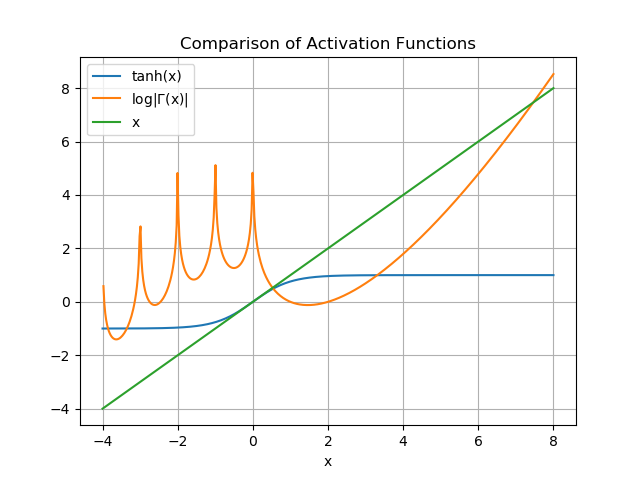
\includegraphics[scale=1]{ActivationFunctions}
\caption{Plot of three functions for shape comparison. $\log |\Gamma(x)|$ is plotted as the function $\log \Gamma(x)$ becomes complex for $x<0$, the two functions agree for $x \ge 0$. For comparison $\tanh(x)$ and the identity line are plotted. The identity line represents ReLU and ELU activation functions for $x>0$. }
\label{fig:activation}
\end{figure}

\subsection{A Top Down Solution}
We can then plausibly start from the top down and construct a general (vectorised) form for the log theoretical fingerprint which is just 
\begin{equation}
\log \mathcal{M}_D[f(\mathbf{x})](\mathbf{s}) = \Delta + \sum_{k=1}^{N_+} w_k \log \Gamma( \boldsymbol\alpha_k \cdot \mathbf{s} + \boldsymbol\beta_k) + \sum_{k=1}^{N_-} w_k \log \Gamma(\mathbf{1} - \boldsymbol\gamma_k \cdot \mathbf{s} - \boldsymbol\delta_k),
\end{equation}
for new vectorised parameters $\boldsymbol\alpha, \boldsymbol\beta, \boldsymbol\gamma, \boldsymbol\delta$, where $N_+$ and $N_-$ control the number of terms of each form. If the weights are restricted to $w_k \in \{-1,1\}$, then the solution does not invoke the parameters analogous to $\mathbf{i,j,k,l}$ in table \ref{tab:main}, if the corresponding scale parameters $\boldsymbol \alpha_k$ and $\boldsymbol\gamma_k$ are set to zero then the solution is restricted to generalised hypergeometric series. By minimising the squared difference in the log theoretical fingerprint, and the log numeric fingerprint the parameters within the log-gamma functions are solved for. If the settings are right it will be possible to write a concise (multivariate) series expansion for the fitted function by interpreting it in terms of the GRMT. The benefit of this top down form is that weights can approach zero if there are too many log-gamma terms, although this may require additional regularisation terms in the loss function and further development for best practices for training.

\subsection{Gradients}
The log-gamma function is (functionally) well suited to extracting gradients and higher order derivatives. We have that $n^{th}$ derivative is given by
$$
\frac{\partial^n}{\partial \alpha_{ij}^n} \sum_{k=1}^{N} w_k \log \Gamma( \boldsymbol\alpha_k \cdot \mathbf{s} + \boldsymbol\beta_k) = w_k s_j^n \psi^{(n-1)}( \boldsymbol\alpha_k \cdot \mathbf{s} + \boldsymbol\beta_k)
$$
where $\psi^{(k)}(x)$ is the polygamma function. This means that closed forms could plausibly be written for high order differential routines. Once again this may be subject to optimisation over complex numbers and polygamma functions do extend to the complex plane.


\subsubsection{Analogy to Deep Networks}
We very briefly consider the extension to neural networks with more than one layer. Unfortunately, some functions have complicated fingerprints which do not consist of only gamma functions and their reciprocals. Take for example the surprisingly simple function $f(x_1) = e^{-x^2_1/3 - x_1}$, whose Mellin transform is given by \begin{equation}
\mathcal{M}[f(x_1)](s_1) = \frac{3^{s_1/2}\Gamma(s_1)}{2^{s_1}}U\left(\frac{s_1}{2},\frac{1}{2},\frac{3}{4}\right)
\end{equation}
where $U(a,b,x)$ is the Tricomi hypergeometric function. The nice property of the Mellin transform is that this hypergeometric function is still related to gamma functions. If we include a `virtual' parameter $x_2$, such that when $x_2=1$ the previous expression is preserved, we could perform a second Mellin transform such as 
\begin{equation}
\mathcal{M}_{x_2 \to s_2}[\mathcal{M}_{x_1 \to s_1}[f(x_1)]](s_1,s_2) =\mathcal{M}_{x_2 \to s_2}\left[ \frac{3^{s_1/2}\Gamma(s_1)}{2^s_1}U\left(\frac{s_1}{2},\frac{1}{2},\frac{3x_2}{4}\right) \right] = 3^{(s_1-2s_2)/2}\Gamma\left(\frac{s_1}{2}-s_2\right)\Gamma(2s_2),
\end{equation}
where we now see the right-hand side is comprised of gamma functions, and powers of constants in a way that is representable as a two-dimensional Mellin transform
\begin{equation}
\mathcal{M}_2[f(x_1,x_2)]](s_1,s_2) = 3^{\begin{bmatrix} \frac{1}{2} & -1 \end{bmatrix}\cdot\begin{bmatrix} s_1 \\ s_2 \end{bmatrix}} \Xi \left[\begin{bmatrix} \frac{1}{2} & -1 \\ 0 &  2\end{bmatrix}\begin{bmatrix} s_1 \\ s_2 \end{bmatrix}  \right].
\end{equation}
Using the above \emph{iterated} process we can construct an analogy to a deeper neural network, where each (hidden) layer requires another Mellin transform with respect to a virtual parameter. If this could be generalised and implemented seamlessly, the algorithm would be able to detect a much wider range of functions and distributions. However, the analogy cannot be realised, because each Mellin transform was equivalent to a sampling operation from some distribution, and virtual distribution is not well defined from the numeric data.\\

In this vein, Rathie et al. have devloped a Y-function, where the gamma functions are replaced by Tricomi hypergeometric functions \cite{Rathie2013}. The significance of this is that these hypergeometric functions themselves can be expressed through an inverse Mellin transform. These advanced functions may be closer in analogy to an iterated, or second layer, requiring a Mellin Transform of the fingerprint, to give the \textbf{fingerprint of the fingerprint}. Rathie goes on to define functions which replace the gamma functions with other generalised functions including incomplete gamma functions and Fox-H functions. We leave the development of this idea for future work, but if these further representations could be harnessed, many more functions could be recognised. It may be possible to fit not only log-gamma functions, but also log-hypergeometric functions to the moments. The downside of this is that high order hypergeometric functions are harder to fit due to varying domains of convergence and analytic continuation and they can be numerically expensive to evaluate. 

\section{Conclusions}
We have presented a framework for representing and working with unknown functions with an aim to applying machine learning techniques and tools to mathematically classify unknown distributions. We call this process \emph{exact learning}, because if the resulting parameters of the fitting process are understood in the right context it may be possible to reconstruct a formula for the unknown distribution. We developed a few ideas within this framework including the notion of a `fingerprint' of a function in a transformed space which is easier to traverse when attempting to identify the function. We used the Mellin transform and its inverse as a tool to switch between the representation spaces, and we noted an extensive hierarchy of functions exists in the literature whose fingerprints are comprised of gamma functions, with shift, scale and power parameters along with constants and scaled constant terms. We believe these functions to be a promising starting point to build exact learning algorithms, interpret the outcomes in a human readable way and categorise and document unknown numeric solutions. We have shown that multivariate analogues exist for these functions and methods, and indicated that the exact learning method may scale to high dimensional numeric data and requires relatively few parameters to learn the fingerprint.\\

We found that a multivariate extension of the most generalised function can take a relatively compact form, and the log of the theoretical fingerprint begins to resemble an unsupervised network. A natural analogy exists between a single layer neural network with a `log-gamma' activation function or basis function. There are also possible extensions to deeper networks with more layers and this new perspective may be a step towards explaining how neural networks work and interpreting the coefficients and weights in the same way that the hierarchy of functions is developed. The log-gamma activation function has particularly nice derivatives, but a complex branch structure will undoubtedly require new techniques for efficient training and optimisation.\\

Further developments could include the addition of polygamma terms as well as gamma terms to the fingerprint which would relate to series expansions containing powers of logarithms as well as monomial terms. One could also imagine a larger network which is comprised of multiple exact learning `units' containing sums of terms, products of terms and compositions of functions. Sums of functions would be trivial to implement, but further mathematical developments would be required train such networks for products including Mellin convolution and development of the equivalent of a Ramanujan master theorem for arbitrary trees of binary operations on functions.\\

The supplementary materials contain extended discussion on future work and the limitations of the methods we presented here. We also implemented some basic versions of the exact learning algorithm along with a basic method for fitting the fingerprints using complex numbers. The key limitations of the method presented here is that functions are currently restricted to the domain $[0,\infty)^n$, and must be representable by the hierarchy of functions described by a Mellin-Barnes integral, which as we showed does not cover even some simple examples of functions. The method used for sampling moments for these prototypes is crude, and the results are currently demonstrable for bound `distribution' like functions for which the whole domain has been sampled. With numeric Mellin transforms, and advanced sampling and training methods we hope to see `exact learning' evolve into a more sophisticated method which makes useful discoveries in many fields of science. We believe the representation presented here is a good starting point for further developments.


\section{Acknowledgements}
B. W. J. Irwin acknowledges the majority of the research was made during his time in the EPSRC Centre for Doctoral Training in Computational Methods for Materials Science for funding under grant number EP/L015552/1.


\bibliography{bibliography}{}
\bibliographystyle{unsrt}


\end{document}